\documentclass[aspectratio=169,10pt]{beamer}
\usepackage[utf8]{inputenc}
\usepackage[T1]{fontenc}
\usepackage{ulem}
\usepackage{xcolor}
\usepackage{listings}
\usepackage{tikz}
\usepackage{multimedia}
\usepackage{array}
\usepackage{textcomp}
\usepackage{underscore}
\lstset{
  backgroundcolor=\color{white},   % choose the background color; you must add \usepackage{color} or \usepackage{xcolor}; should come as last argument
  basicstyle=\footnotesize\ttfamily,        % the size of the fonts that are used for the code
  breakatwhitespace=false,         % sets if automatic breaks should only happen at whitespace
  breaklines=true,                 % sets automatic line breaking
  captionpos=b,                    % sets the caption-position to bottom
  commentstyle=\color{gray},    % comment style
  deletekeywords={...},            % if you want to delete keywords from the given language
  escapeinside={\%*}{*)},          % if you want to add LaTeX within your code
  extendedchars=true,              % lets you use non-ASCII characters; for 8-bits encodings only, does not work with UTF-8
  frame=single,                    % adds a frame around the code
  keepspaces=true,                 % keeps spaces in text, useful for keeping indentation of code (possibly needs columns=flexible)
  keywordstyle=\color{blue},       % keyword style
  language=bash,                 % the language of the code
  morekeywords={*,...},            % if you want to add more keywords to the set
  numbers=left,                    % where to put the line-numbers; possible values are (none, left, right)
  numbersep=5pt,                   % how far the line-numbers are from the code
  numberstyle=\tiny\color{gray},   % the style that is used for the line-numbers
  rulecolor=\color{black},         % if not set, the frame-color may be changed on line-breaks within not-black text (e.g. comments (green here))
  showspaces=false,                % show spaces everywhere adding particular underscores; it overrides 'showstringspaces'
  showstringspaces=false,          % underline spaces within strings only
  showtabs=false,                  % show tabs within strings adding particular underscores
  stepnumber=1,                    % the step between two line-numbers. If it's 1, each line will be numbered
  stringstyle=\color{teal},        % string literal style
  tabsize=2,                       % sets default tabsize to 2 spaces
  title=\lstname,                  % show the filename of files included with \lstinputlisting; also try caption instead of title
  columns=fullflexible,            % Less spacing between characters
  literate={á}{{\'a}}1 {ã}{{\~a}}1 {é}{{\'e}}1,
}
\lstdefinestyle{base}{
  langage=bash,
  moredelim=**[is][\color{red}]{@}{@},
}

\usetheme{Rochester}
\beamersetuncovermixins{\opaqueness<1>{25}}{\opaqueness<2->{15}}
\newcommand{\light}[1]{\sout{\textcolor{gray}{#1}}}
\newcommand{\shell}[1]{\textcolor{brown}{#1}}
\newcommand{\cont}[1]{\textcolor{orange}{#1}}
\newcommand{\err}[1]{\textcolor{red}{#1}}

%\definecolor{orange_smile}{RGB}{225, 128, 84}
%\setbeamercolor*{frametitle}{parent=orange_smile}

\definecolor{UBCblue}{rgb}{0.04706, 0.13725, 0.26667} % UBC Blue (primary)
%\definecolor{OrangeSMILE}{rgb}{0.88235, 0.50196, 0.32941} % UBC Blue (primary)

\usecolortheme[named=UBCblue]{structure}



\AtBeginSection[] % Do nothing for \section*
{
\begin{frame}
  \frametitle{Outline}
  \tableofcontents[currentsection]
\end{frame}
}

% #############################################################################
%   BEGIN DOCUMENT
% #############################################################################

%\title{THE LINUX SHELLS \\ Use, Understand, Customize}
\title{THE LINUX SHELLS}
\subtitle{Use, Understand, Customize}
%\author{Rayan Mac}
\author[shortname]{Rayan Mac}
\date{2020-03-25}
\titlegraphic{
\includegraphics[scale=0.02]{./images/logoCC_minimalist}}
\begin{document}

% =============================================================================
%   Title / Table of contents

\begin{frame}
  \titlepage
\end{frame}

\section*{Context}

\setbeamercovered{invisible}

\begin{frame}[c]
    \begin{center}
        \huge What is a shell ?\\
        \pause
        \vspace{\baselineskip}
        \Large A command interpreter
        \vspace{\baselineskip}
        \begin{figure}[h]
            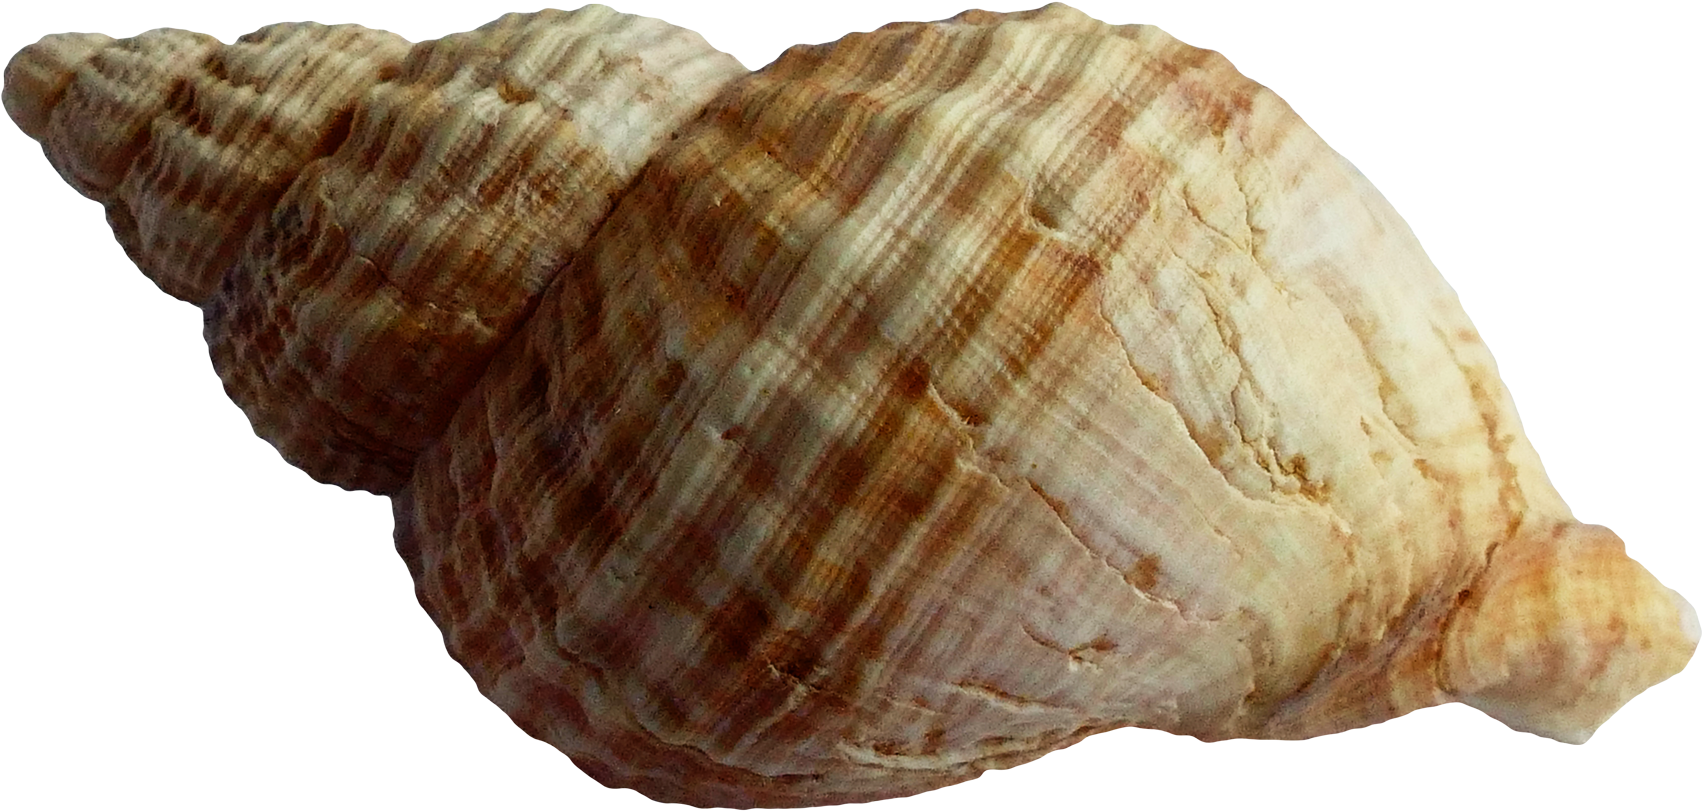
\includegraphics[scale=0.07]{./images/SeaShellOK}
        \end{figure}
    \end{center}
\end{frame}

% Back to normal
\setbeamercovered{transparent}

% =============================================================================
%   PART 1
%

\begin{frame}[c]
    %\frametitle{A first slide}
    \begin{center}
        % \huge PART 1 : The shell way of life (alternative)
        \huge PART 1 : Living like a shell
    \end{center}
\end{frame}

\section{Three stages}

\subsection{Initialization}

\begin{frame}
  \frametitle{Initialization}
    \begin{figure}[h]
        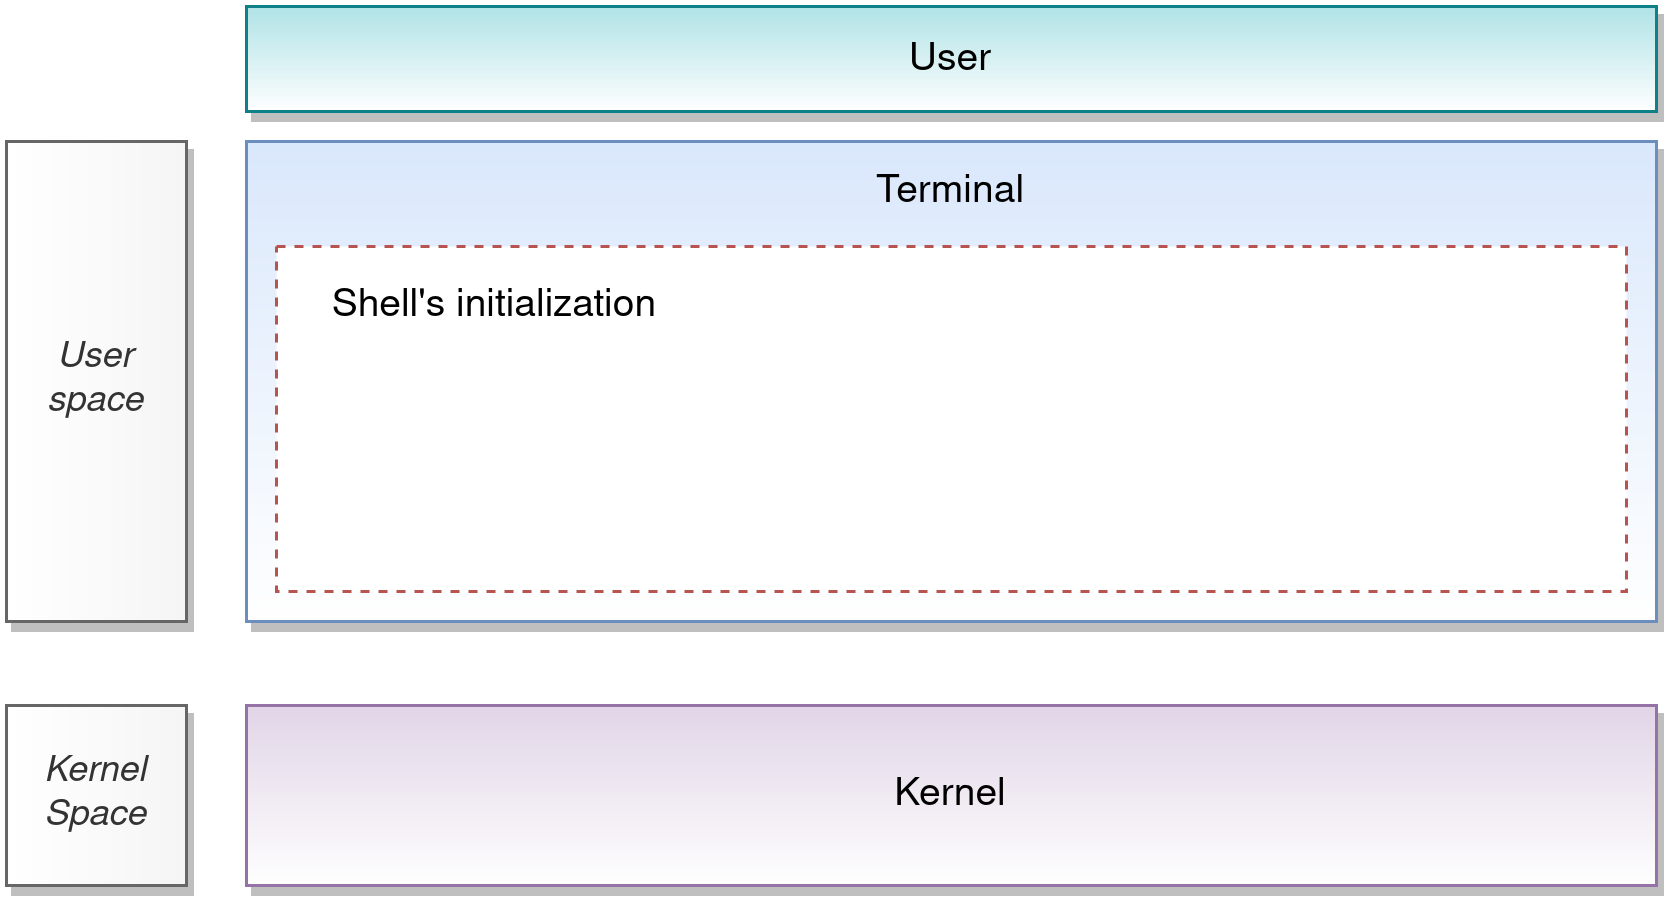
\includegraphics[scale=0.8]{./images/ShellStepsBeforeInit}
    \end{figure}
\end{frame}

\begin{frame}[fragile]
  \frametitle{Initialization - Getting environment from start-up files (Bash)}
    \small{
        \vspace{\baselineskip}
  Login shells
  \begin{itemize}
    \item After an immediate login, prepended with a `-' character (echo \$0)
    \item Read:
      System login scripts : /etc/profile \\
      User login scripts : \~{}/.bash\_profile, \~{}/.bash\_login, or \~{}/.profile (the first existing file)
  \end{itemize}

  \vspace{\baselineskip}

  Non login shells
  \begin{itemize}
    \item Started on demand, when user has already logged in
    \item Only read \~{}/.bashrc
  \end{itemize}

  \vspace{\baselineskip}

Common practice:

    \begin{lstlisting}
    # ~/.bash_profile
    [[ -f ~/.bashrc ]] && . ~/.bashrc
    \end{lstlisting}
}

\end{frame}

\begin{frame}[fragile]
  \frametitle{Initialization - Great reminders}
  Man bash:
  \vspace{\baselineskip}
    \begin{lstlisting}[basicstyle=\scriptsize,]
      INVOCATION
      A login shell is one whose first character of argument zero is a -, or one started with the --login option.
      [...]
      When  bash  is  invoked  as an interactive login shell, or as a non-interactive shell with the --login option, it first reads and executes commands
      from the file /etc/profile, if that file exists.  After reading that file, it looks for ~/.bash_profile, ~/.bash_login, and ~/.profile, in that or‐
      der,  and reads and executes commands from the first one that exists and is readable.  The --noprofile option may be used when the shell is started
      to inhibit this behavior.
    \end{lstlisting}
\end{frame}

\begin{frame}[fragile]
  \frametitle{Initialization - Great reminders}
    Source code:
    \vspace{\baselineskip}
    \begin{lstlisting}[basicstyle=\scriptsize,]
      if (login_shell < 0 && posixly_correct == 0)
      {
        /* We do not execute .bashrc for login shells. */
        no_rc++;

        /* Execute /etc/profile and one of the personal login shell
           initialization files. */
        if (no_profile == 0)
        {
            maybe_execute_file (SYS_PROFILE, 1);

            if (act_like_sh)▸·/* sh */
                maybe_execute_file ("~/.profile", 1);
            else if ((maybe_execute_file ("~/.bash_profile", 1) == 0) &&
                    (maybe_execute_file ("~/.bash_login", 1) == 0))▸··/* bash */
                maybe_execute_file ("~/.profile", 1);
        }
        sourced_login = 1;
      }
    \end{lstlisting}
\end{frame}

\begin{frame}
  \frametitle{Initialization - The shell execution environment}

  The shell has an execution environment, which consists of the following:

  \vspace{\baselineskip}

  \begin{itemize}

    \item OPENED FILES inherited by the shell at invocation
    \item CURRENT WORKING DIRECTORY as set by cd
    \item FILE CREATION MODE MASK, as set by umask
    \item CURRENT TRAPS, set by trap
    \item ENVIRONMENT AND SHELL VARIABLES
    \item SHELL FUNCTIONS AND ALIASES
    \item VARIOUS PROCESS IDs, those of background jobs, \$\$ and \$PPID, etc...
    \item OTHER OPTIONS enabled by 'set' or 'shopt' builtins
  \end{itemize}
\end{frame}

\begin{frame}

    \frametitle{Some useful set options}

    \begin{table}[]
        \small
        \begin{tabular}{|l|l|}
            \hline
            \begin{tabular}[c]{@{}l@{}}set -e\\ set -o errexit\end{tabular} &
            Exit immediately if a simple command exits with a non-zero status \\ \hline
            \begin{tabular}[c]{@{}l@{}}set -n\\ set -o noexec\end{tabular} &
            \begin{tabular}[c]{@{}l@{}}Read commands but do not execute them;\\ this can be used to check a script for syntax errors.\end{tabular} \\ \hline
            \begin{tabular}[c]{@{}l@{}}set -u\\ set -o nounset\end{tabular} &
            \begin{tabular}[c]{@{}l@{}}Treat unset variables as an error when performing parameter expansion.\end{tabular} \\ \hline
            \begin{tabular}[c]{@{}l@{}}set -v\\ set -o verbose\end{tabular} &
            Print shell input lines as they are read. \\ \hline
            \begin{tabular}[c]{@{}l@{}}set -x\\ set -o xtrace\end{tabular} &
            \begin{tabular}[c]{@{}l@{}}Print a trace of simple commands and their arguments\\after they are expanded and before they are executed.\end{tabular} \\ \hline
        \end{tabular}
    \end{table}

\vspace{\baselineskip}
Common practice in writing and debugging: set -eu

\end{frame}

\subsection{Command Parsing}

\begin{frame}
  \frametitle{Command Parsing}
    \begin{figure}[h]
        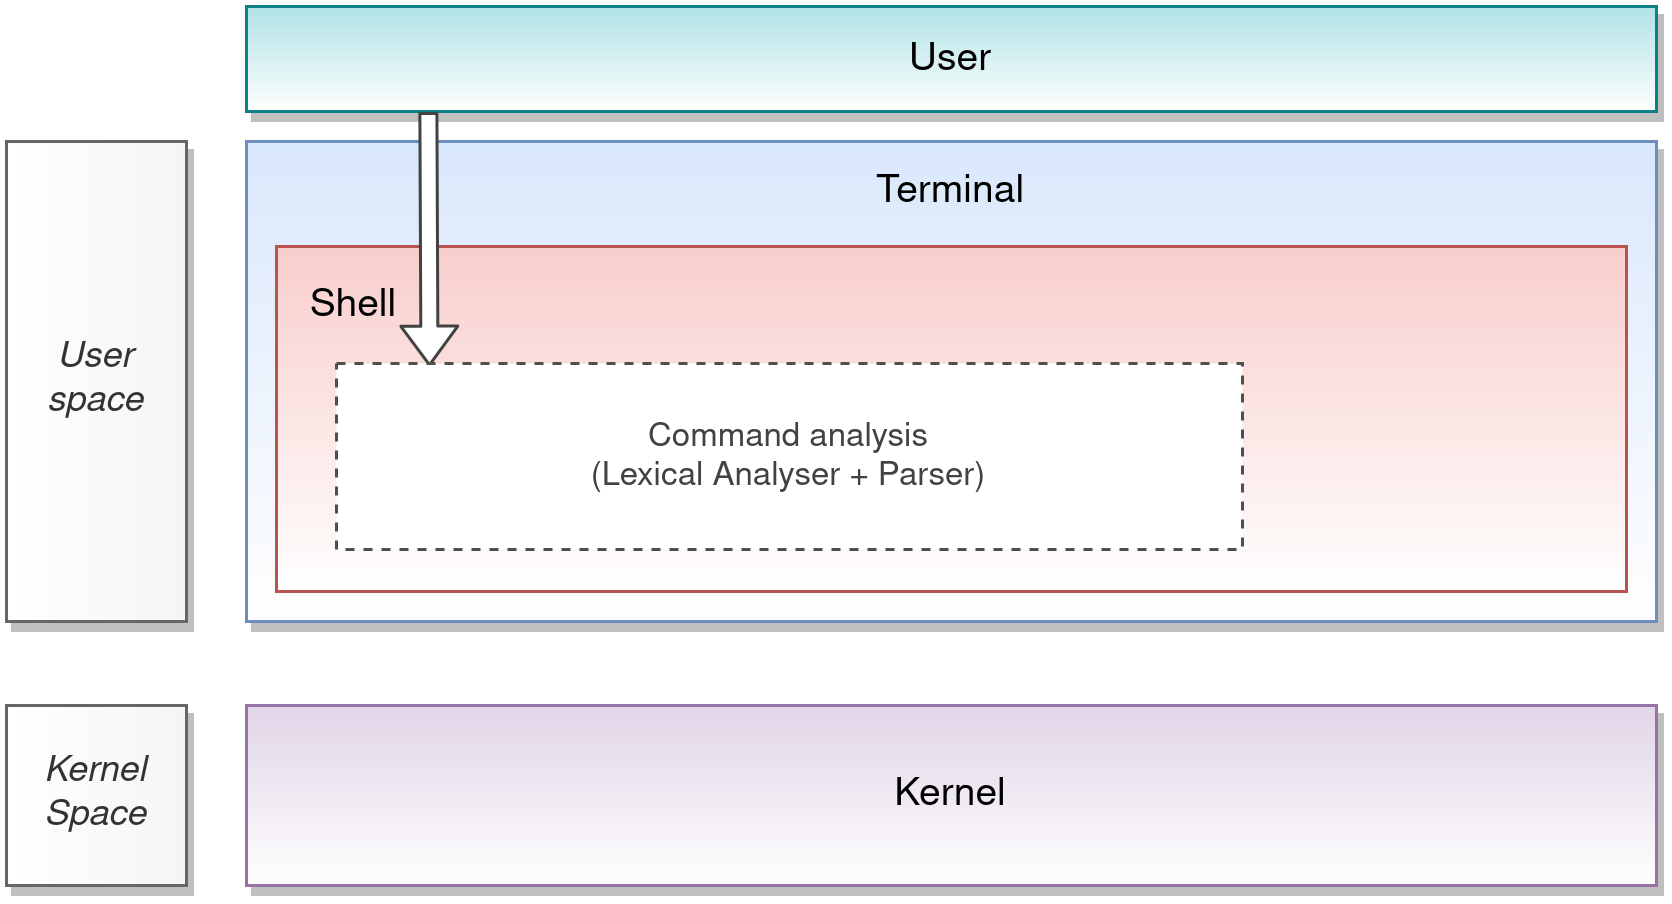
\includegraphics[scale=0.8]{./images/ShellStepsBeforeAnalysis}
    \end{figure}
\end{frame}

\begin{frame}
  \frametitle{Command Parsing - Input Analysis}
    \normalsize{
  \begin{enumerate}
    \item Token Recognition (words are split on whitespaces)
    \item Substitution (parameter and command)
    \item Field splitting (words are split on \$IFS variable)
    \item Globbing
    \item Execution (commands and control sructures)
  \end{enumerate}
  }
\end{frame}

\begin{frame}
  \frametitle{Going deeper: The similarities with compilers}

    \begin{figure}
        
\includegraphics[scale=0.85]{./images/LexerParserAST}
    \end{figure}

    \vspace{\baselineskip}

    \underline{Lexer} (Lexical Analyser): Breaks the input string to a series of token through lexical analysis\\
    \underline{Parser}: Grammatical analysis of the tokens to build the AST\\
    \underline{AST} (Abstract Syntax Tree) : A tree-like data structure that holds tokens and operations in order of the execution
\end{frame}

% For quizz time we will hide answers
\setbeamercovered{invisible}

% Example n°1
\begin{frame}[fragile]
  \frametitle{Quiz time ! What is the output of these commands ?}  %PRACTCAL ?

  \begin{lstlisting}
  IF=if
  $IF true; then echo "hello world"; fi
  \end{lstlisting}

  \pause
  Output: Error, unexpected token

\end{frame}

% Example n°2
\begin{frame}[fragile]
  \frametitle{Quiz time ! What is the output of these commands ?}

  \begin{lstlisting}
  file="foo.txt"  # foo.txt not being empty
  head -n 10 ${file} > {file}
  cat ${file}
  \end{lstlisting}

  \pause
  Output: Nothing
\end{frame}

% Example n°3
\begin{frame}[fragile]
  \frametitle{Quiz time ! What is the output of these commands ?}

  \begin{lstlisting}
  STR="Hello        :great:world"
  echo $STR
  IFS=':' ; echo $STR
  \end{lstlisting}

  \pause
  Output:
  \begin{verbatim}
  Hello :great:world
  Hello         great world
  \end{verbatim}

  More challenges at https://mywiki.wooledge.org/BashPitfalls
\end{frame}

% Back to normal
\setbeamercovered{transparent}

\subsection{Execution}

\begin{frame}
  \frametitle{Execution}
    \begin{figure}[h]
        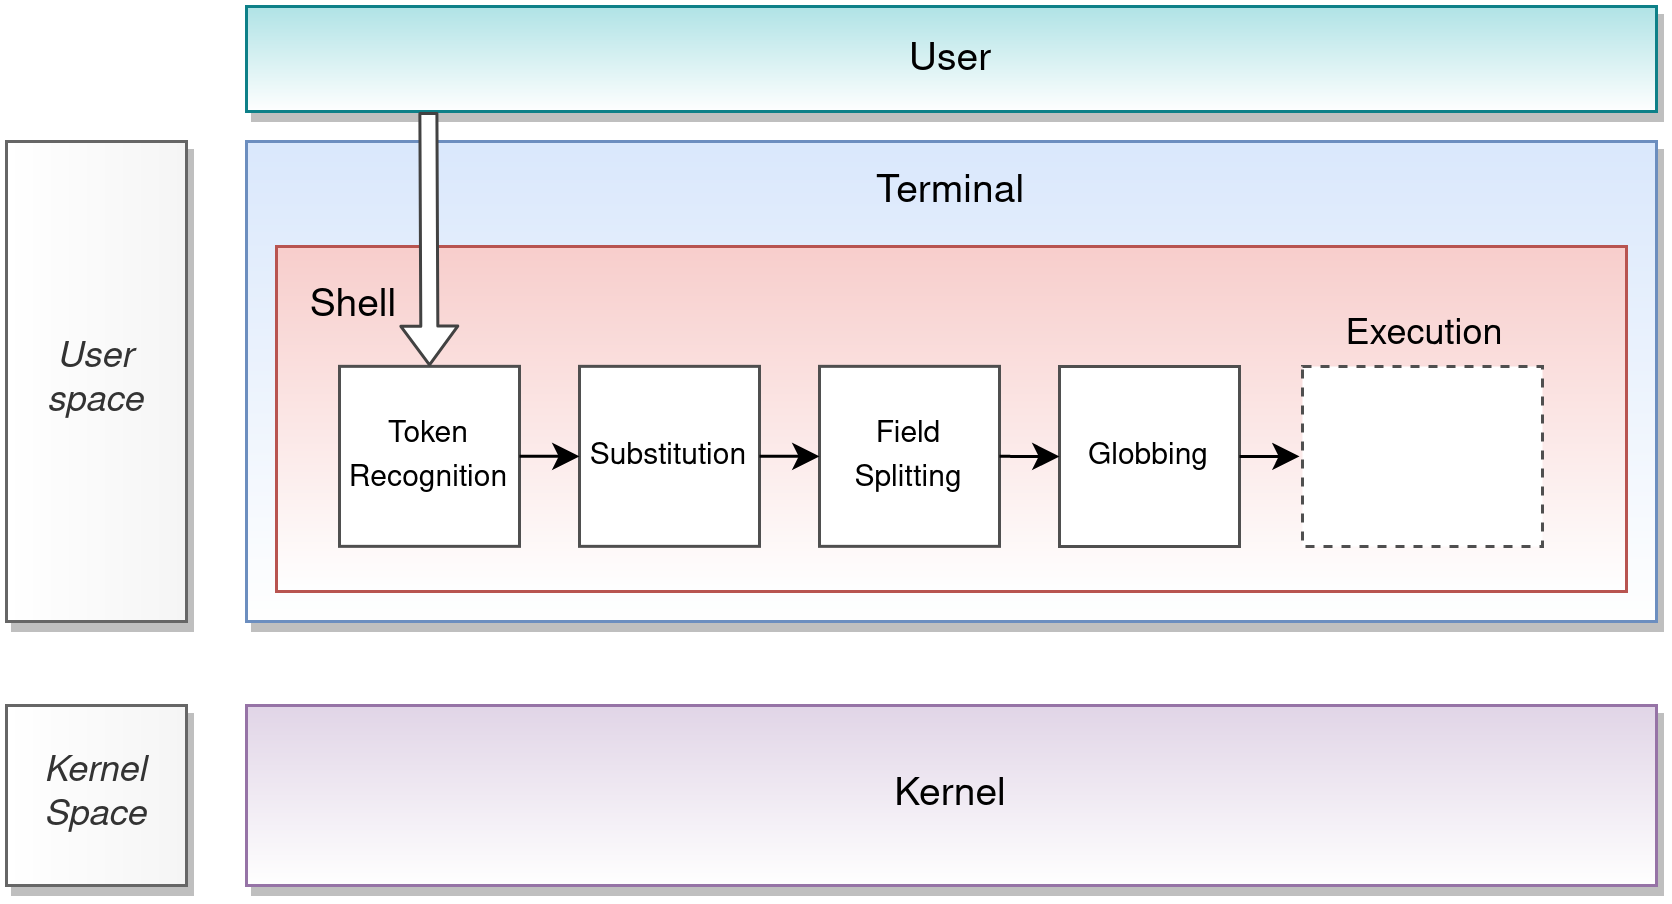
\includegraphics[scale=0.8]{./images/ShellStepsBeforeExecution}
    \end{figure}
\end{frame}

\begin{frame}
  \frametitle{Execution - External commands}
    \begin{center}
        {\huge fork / execve}
    \end{center}
\end{frame}

\begin{frame}[fragile]
  \frametitle{Execution - Tracking with strace}
  \$ strace bash\\
  \$ cat foo.txt > bar.txt

  \vspace{\baselineskip}

    \begin{lstlisting}[basicstyle=\scriptsize,]
    [...........]
    open("bar.txt", O_WRONLY|O_CREAT|O_TRUNC, 0666) = 3
    dup2(3, 1)                        = 1
    close(3)                          = 0
    execve("/bin/cat", ["cat", "foo.txt"], [/* 47 vars */]) = 0
    [...........]
    open("foo.txt", O_RDONLY)         = 3
    [...........]
    read(3, "Hello world\n", 131072)  = 12
    write(1, "Hello world\n", 12)     = 12
    read(3, "", 131072)               = 0
    munmap(0x7f5cd9dcf000, 139264)    = 0
    close(3)                          = 0
    close(1)                          = 0
    close(2)                          = 0
    exit_group(0)                     = ?
    +++ exited with 0 +++
    \end{lstlisting}
\end{frame}

\begin{frame}
    \frametitle{Execution - Built-ins}

    Executed directly in the shell itself
    \begin{itemize}
        \item Faster execution
        \item Can modify the shell's context
    \end{itemize}

    \vspace{\baselineskip}

    Check nature of a command: \lstinline{$ type <cmd>}
    \newline
    Display list of shell built-ins: \lstinline{$ help}
\end{frame}


\begin{frame}
  \frametitle{Overall process}
    \begin{figure}[h]
        \includegraphics[scale=0.8]{./images/ShellStepsGlobal}
    \end{figure}
\end{frame}

\begin{frame}[c]
    \begin{center}
        \huge PART 2 : A sea of shells
    \end{center}
\end{frame}

\section{A brief of history}
\subsection{From sh to *sh}

\begin{frame}
    \frametitle{A brief of history}

    1971 : The Thompson shell
    \begin{itemize}
        \item First UNIX shell
        \item No scripting
        \item 900 lines of C source
    \end{itemize}

    \vspace{\baselineskip}

    1977 : Bourne Shell (sh)
    \begin{itemize}
        \item Command interpreter AND scripting language
        \item [+] Variables and command substitution
        \item [+] Control structures and loop
    \end{itemize}

\end{frame}

\begin{frame}
    \frametitle{A brief of history}

    1978 : The C shell (csh) then Tenex C shell (tcsh)
    \begin{itemize}
        \item Scripting language "similar" to the C language
        \item Incompatible with sh
        \item [+] Command history in interactive use
    \end{itemize}

    \vspace{\baselineskip}

    1983: The Korn shell (ksh)
    \begin{itemize}
        \item Proprietary software until 2000 (then Common Public Licence)
        \item [+] Associative arrays
        \item [+] Floating point arithmetic
    \end{itemize}

\end{frame}

\begin{frame}
    \frametitle{A brief of history}

    1989: The Almquist Shell (ash)
    \begin{itemize}
        \item A lightweight sh version
        \item Only implements POSIX features
        \item The Busybox's shell
    \end{itemize}

    \vspace{\baselineskip}

    1989: The Bourne Again Shell (bash)
    \begin{itemize}
        \item GNU GPLv3
        \item Enhanced version of sh
        \item Comes packaged as part of GNU
    \end{itemize}

\end{frame}

\begin{frame}
  \frametitle{And many more !}
    \begin{figure}[h]
        \includegraphics[scale=0.5]{./images/shellsHistorySmaller}
    \end{figure}
\end{frame}

\subsection{Portability concerns}

\begin{frame}
    \frametitle{What about compatibility ?}
    1992: Definition of what a POSIX shell shall be

%    \newline
    \vspace{\baselineskip}

    When portability matters, avoid using a shell's specific feature\\
    Try to execute your script using the bare /bin/sh (if existing)

%    \newline
    \vspace{\baselineskip}

    Otherwise:
    \begin{itemize}

        \item POSIX shell standard available online
        \item Tools exist to assess POSIX compliance:
            \begin{itemize}
                \item[--] The ash/dash (and posh ?) shell
                \item[--] 'shellcheck' utility
            \end{itemize}
    \end{itemize}
\end{frame}

\subsection{Today's shells}

\begin{frame}[c]
    \begin{center}
        \huge What to expect from a shell today ?
    \end{center}
\end{frame}

\begin{frame}[fragile]
  \frametitle{Bash 5.0 Release, what's new ?}

    2019/01/07: v4.4 \textrightarrow{} v5.0 (stable)

    \vspace{\baselineskip}

  \begin{itemize}
      \item Bugfixes (potential out-of-bounds memory errors, ...)
      \item New shell variables: BASH\_ARGV0, EPOCHSECONDS et EPOCHREALTIME
      \item Shell option `globasciiranges' enabled by default (ensure [a-d] == [abcd])
      \item New options for the `history' built-in
          \begin{verbatim}history -d <start>-<end>\end{verbatim}
      \item \begin{verbatim}[...]\end{verbatim}
  \end{itemize}

\end{frame}

\begin{frame}
    \frametitle{More interactive features ? [Demo time]}
  Examples of the fish and zsh shells:
    \begin{figure}[h]
        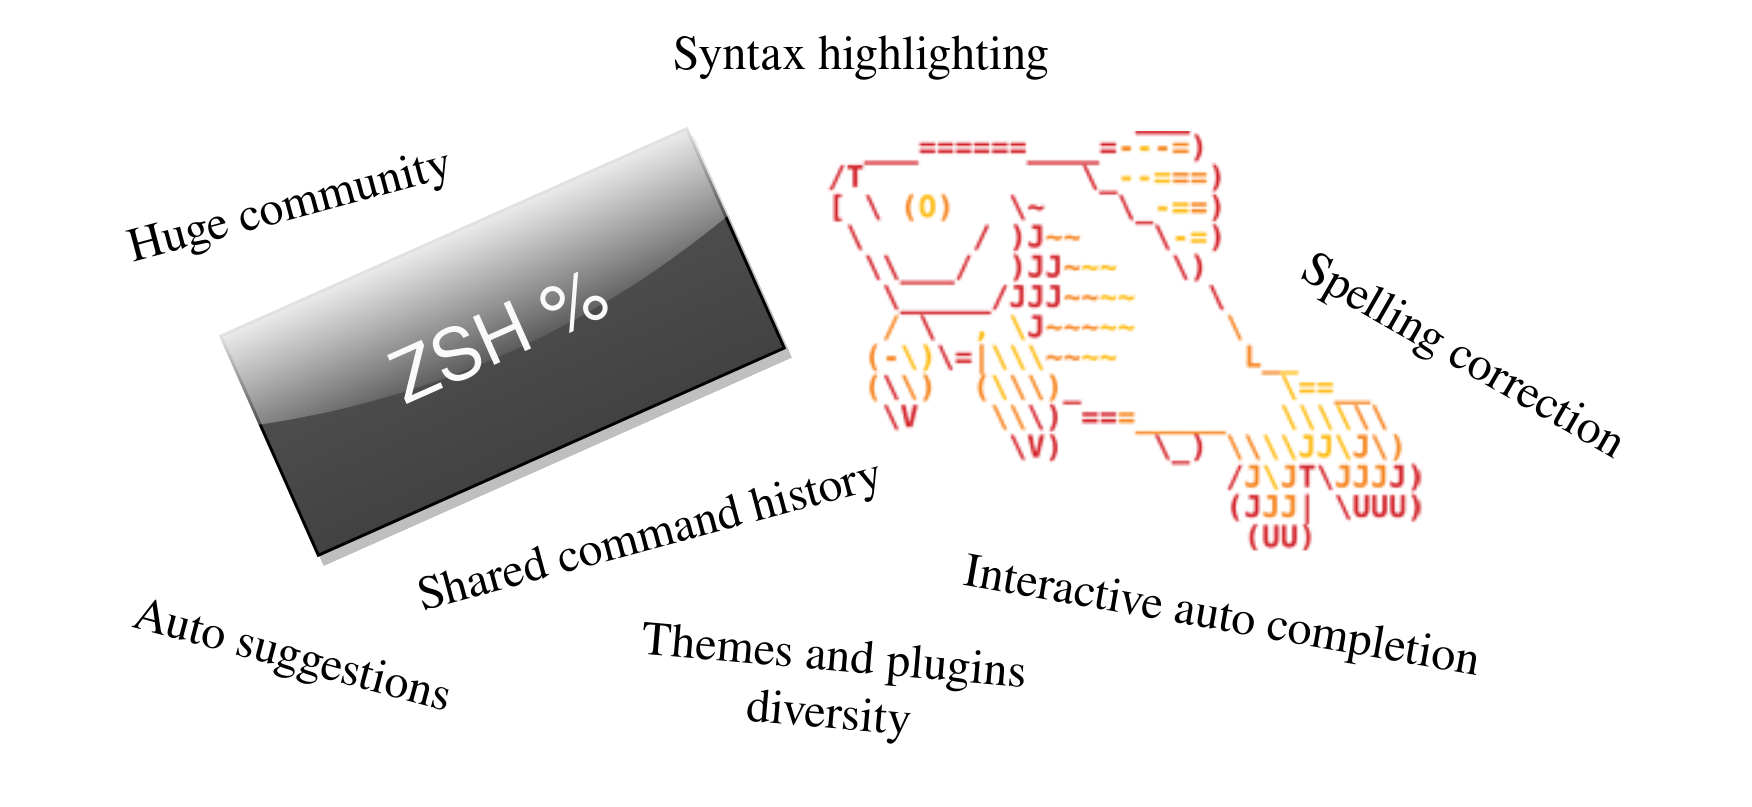
\includegraphics[scale=0.8]{./images/zshFish}
    \end{figure}
\end{frame}

\begin{frame}[fragile]
  \frametitle{Which shell to use or test scripts with ?}

  Some suggestions:
  \vspace{\baselineskip}

    \begin{itemize}
        \item Embedded: ash (making local tests with dash if more convenient)
        \item Portability: sh when available (will lead you to a shell considered as POSIX)
        \item Daily use: (bash|ksh|fish|zsh|.*)
    \end{itemize}
\end{frame}


\begin{frame}
  \frametitle{CONCLUSION}
    \large{
  USE your shell efficiently, tweaking options when helpful \\
  \vspace{\baselineskip}
  UNDERSTAND how it works to improve your scripting \\
  \vspace{\baselineskip}
  CUSTOMIZE it to your needs and enjoy !
  }
\end{frame}

\begin{frame}[c]
    \begin{center}
        \Huge Thanks for your attention \\ \huge Let's share !
    \end{center}
\end{frame}

\begin{frame}
  \frametitle{References and useful resources}
Books:
    \begin{itemize}
\item Peter Seebach - "Beginning Portable Shell Scripting"
\item Christophe Blaess - "Shells Linux et Unix"
\item Arnold Robbins \& Nelson H.F. Beebe - Classic Shell Scripting; // O'Reilly Edition
    \end{itemize}

\vspace{\baselineskip}

Links:
    \begin{itemize}
        \item https://pubs.opengroup.org/onlinepubs/9699919799/utilities/V3\_chap02.html
        \item https://developer.ibm.com/tutorials/l-linux-shells/\#artrelatedtopics
        \item http://www.aosabook.org/en/bash.html
        \item https://github.com/Swoorup/mysh
    \end{itemize}
\end{frame}

\end{document}
